% Choptuik's critical solution at large dimension: the physics paper. Build: see Makefile (pdflatex twice).
% Companion: the mathematics paper in ../math/ (cited as [math]).
\documentclass[aps,prd,onecolumn,superscriptaddress,nofootinbib,10pt]{revtex4-2}
\usepackage{amsmath,amssymb}
\usepackage{graphicx}
\usepackage{booktabs}
\usepackage{dcolumn}
\usepackage{xurl}
\usepackage[colorlinks=true,linkcolor=blue,citecolor=blue,urlcolor=blue]{hyperref}

\newcommand{\Dinf}{\Delta_\infty}
\newcommand{\eps}{\varepsilon}

\begin{document}

\title{Choptuik's echo period and critical exponent at large dimension:\\
evidence for $\Delta_\infty = 1.64389375$ and an $r^2$-shift symmetry behind $\gamma_\infty = 1/2$}

\author{Nathan Moinvaziri}
\email{nathan@nathanm.com}
\affiliation{Independent researcher}
\date{October 2026; unreviewed draft}

\begin{abstract}
% TODO: abstract (written last).
\end{abstract}

\maketitle

% OUTLINE
% I.   Introduction: the problem, prior numerics and large-D work (credits), what this paper reports, the companion
%      paper [math], conventions (gamma is the radius exponent).
% II.  Equations and numerical method: self-similar equations; the f64 and double-double solvers; checks table;
%      the growth rate as a root of the growth-mode determinant.
% III. Delta(D) and gamma(D) for D >= 4: the rational formula (coefficients, values, figure); comparison with
%      published values (D = 4, the maximum below D = 4, D = 5); physical reading (echo factor, fine-tuning per echo).
% IV.  The limit D -> infinity: held-out tests of analyticity in 1/D; Delta_inf and its planted-truth check; the
%      Delta -> 0 conjecture; closed forms tested; gamma_inf = 1/2 from the data.
% V.   The large-D picture: how the solution scales; a free wave cannot echo and the period is selected beyond all
%      orders (statements, proofs in [math]); the inner region x ~ sqrt(n) and Rozali-Way's heat equation; the
%      r^2-shift and gamma_inf = 1/2; the D = infinity selection rule (conjecture, [math]) and what it reproduces;
%      the next-to-leading-order condition of Ecker, Ecker and Grumiller.
% VI.  Other matter at large D: which models keep the r^2-shift; axion-dilaton and complex scalar (CSS, D <= 80);
%      the sigma-model CSS branch (ends near D = 8.5); the l = 1 multiplet (D <= 9, undecided).
% VII. Discussion: summary, the assumption that the branch stays critical, open problems.
% VIII. How this work was done; data and code.

\section{Introduction}
\label{sec:intro}

Fine-tuning a one-parameter family of initial data for a massless scalar field to the threshold of black-hole formation,
Choptuik found that the evolution approaches a universal critical solution that repeats itself on ever smaller scales: it
is discretely self-similar (DSS) with echo period $\Delta$, and black holes formed just above threshold have a size that
scales as a power of $p - p^*$~\cite{Choptuik1993}. The scaling follows from the critical solution having a single
unstable mode, with exponent $\gamma = 1/\lambda$ for its growth rate $\lambda$~\cite{KoikeHaraAdachi1995}. Throughout,
$\gamma$ is the \emph{radius} exponent, $r_{\rm BH} \propto (p - p^*)^\gamma$; in $D$ spacetime dimensions the mass then
scales as $M \propto (p - p^*)^{(D-3)\gamma}$, and in four dimensions the two exponents coincide. In four dimensions
$\Delta = 3.445452402(3)$~\cite{MartinGarciaGundlach2003} and $\gamma \simeq 0.374$~\cite{Gundlach1997}; see the
review~\cite{GundlachReview2025}.

The dependence on the spacetime dimension $D$ has been studied numerically, mostly at percent-level precision, for
$3.5 \le D \le 14$ (mostly integer $D$)~\cite{GarfinkleCutlerDuncan1999,SorkinOren2005,BlandEtAl2005,BlandKunstatter2007,Bland2007,TavesKunstatter2011},
and to about $10^{-6}$ for continuous $3.05 < D < 5.5$ by Ecker, Ecker, Grumiller and Jechtl~\cite{EckerEtAl2026}, who
find a maximum of $\Delta$ near $D = 3.756$. Large $D$ has been a fruitful limit in gravity~\cite{EmparanHerzog2020}.
For critical collapse, Rozali and Way~\cite{RozaliWay2018} derived the leading-order large-$D$ equations of a
self-gravitating scalar field, observed that they are parabolic with the roles of space and time swapped, and estimated
$\gamma = 1/2$ from the divergence of their oscillating solutions. Clark and Pimentel~\cite{ClarkPimentel2025}
constructed continuously self-similar (CSS) critical solutions at large $D$ by matched asymptotics. Ecker, Ecker and
Grumiller~\cite{EckerEckerGrumiller2026} constructed analytic DSS solutions at large $D$, found that at leading order any
periodic profile with any period solves the equations, and, with~\cite{EckerEtAl2026}, conjectured $\Delta \to 0$ as
$D \to \infty$; they also report the expectation $\gamma \to 1/2$. Bland's thesis~\cite{Bland2007} hypothesised
$\Delta \to 5/2$.

This paper computes $\Delta(D)$ and $\gamma(D)$ to high precision far beyond the dimensions studied before, asks what
happens as $D \to \infty$, and explains what can be explained from the structure of the equations at large $D$. It reports:
\begin{enumerate}
\item $\Delta(D)$ at 857 points $8.25 \le D \le 61.03$ from a double-double (about 32-digit) solver, $\gamma(D)$ at 67
points up to $D = 61$, and both for $4 \le D \le 40$ from an independent double-precision solver; one rational
function of $1/(D-2)$ that reproduces them for all $D \ge 4$; and the comparison with published values, including a
$6\times10^{-5}$ difference at $D = 5$ that the published higher-resolution data trace to resolution
(Sec.~\ref{sec:results}).
\item Held-out tests that support analyticity of $\Delta$ in $1/D$, giving $\Dinf = 1.64389375 \pm 1.5\times10^{-8}$; a
power-law approach to $\Delta = 0$ (exponent at least $0.01$) is excluded and a logarithmic one disfavoured by the data
to $D = 61$; given analyticity, nine constants tested as closed forms for $\Dinf$ are excluded; and $\gamma_\infty = 1/2$
to about $5\times10^{-7}$ (Sec.~\ref{sec:limit}).
\item A physical picture of the large-$D$ limit (Sec.~\ref{sec:picture}). Inside the light cone the echo becomes a weak
free wave, which on its own cannot echo; the period is fixed by effects smaller than every power of $1/D$, in an inner
region at radii of order $\sqrt D$ times the time to the singularity, where the equations become Rozali and Way's
nonlinear heat equation. Its shift symmetry
in $r^2$ gives an exact unstable mode with $\lambda = 2$, which explains $\gamma_\infty = 1/2$ under stated conditions,
and a conjectured selection rule posed there reproduces $\Dinf$ to about $10^{-4}$ and the shape of the echo from the
$D = \infty$ equations alone.
\item Tests on other matter (Sec.~\ref{sec:matter}): for the axion--dilaton and the complex scalar, whose large-$D$
equations keep the $r^2$-shift, $\gamma \to 1/2$ and the selection rule reproduces the limiting frequency; for models
with a centrifugal term, which breaks the symmetry, the computations so far do not decide $\gamma_\infty$.
\end{enumerate}
The theory behind item 3 (the large-$D$ expansion and its Stokes structure, the selection rule with its hypotheses, and a
computer-assisted proof in a model case) is developed in a companion paper~\cite{math}; here we state its results in
physical terms, with the numerical evidence, and refer there for proofs. We assume, without checking it at large $D$,
that the branch we follow remains the critical solution, with a single unstable mode (Sec.~\ref{sec:discussion}).

\begin{figure}[t]
\centering
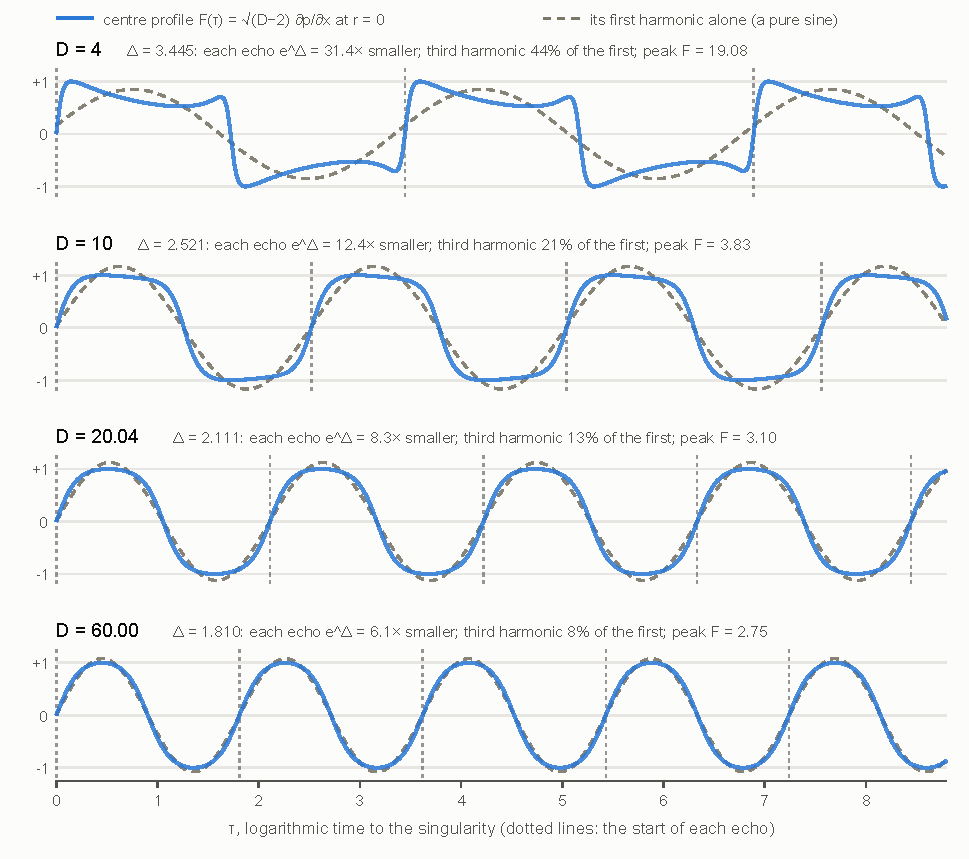
\includegraphics[width=0.92\linewidth]{../figures/echo.pdf}
\caption{The echo across dimensions: the centre slope of the field,
$F(\tau) = \sqrt{D-2}\,\partial_x p$ at $r = 0$, over the same stretch of logarithmic time $\tau$ for $D = 4$, 10, 20
and 60, each scaled to its peak (dashed: its first harmonic). At $D = 4$ the profile is close to a square wave and
each echo is $e^{\Delta} = 31\times$ smaller than the last; at $D = 60$ it is nearly a pure sine and the factor is
$6.1$. The $D = 4$ profile is from the double-precision solver (39 harmonics); the others are double-double
solutions.}
\label{fig:echo}
\end{figure}

% =====================================================================================================
\section{Equations and numerical method}
\label{sec:method}

We use the self-similar radius $x$ (radius over time to the singularity, normalized so that the past light cone of
the singularity is at $x = 1$) and $\tau = -\ln(-t)$, or the phase $\theta = \omega\tau$ with $\omega = 2\pi/\Delta$.
With $n = D - 2$, $p$ and $m$ the (scaled) derivatives of the scalar field along the two radial null directions, $a$
the radial metric function ($b = a^2$) and $c$ the lapse-type function that sets the light cones, the equations are
\begin{align}
x c_x &= (n-1)\,c\,(b-1), &
x b_x &= b\,(p^2+m^2) - (n-1)\,b\,(b-1), \label{eq:E12}\\
x(x-c)\,p_x &= -\omega x\,p_\theta + G p - c p + \tfrac{n}{2}\,c\,(p+m), &
x(x+c)\,m_x &= -\omega x\,m_\theta - G m + c m - \tfrac{n}{2}\,c\,(p+m), \label{eq:E34}
\end{align}
with $G = (n-1)\,c\,(b-1)$, on $0 \le x \le 1$; $p$, $m$ contain only odd harmonics of $\theta$ and $b$, $c$ only even
ones; the solution is regular at $x = 0$, analytic at the past light cone $x = 1$, and $c(1) = 1$ fixes the gauge. The
critical solution is thus computed directly as a periodic boundary-value problem, with $\Delta$ an eigenvalue.

\emph{Double-precision solver} ($4 \le D \le 40$, with points down to $D = 3.7$): spectral multiple shooting in $x$ with
Fourier modes in $\tau$ (23--47 modes), with the integration-step error extrapolated out; near $D = 4$ the points are
extrapolated in the mode count. Above $D \approx 26$ rounding at $10^{-16}$ in the residual moves $\Delta$ by
$10^{-7}$--$10^{-6}$ at $D = 30$--$40$.

\emph{Double-double solver} ($8.25 \le D \le 61.03$): double-double arithmetic (about 32 digits) on SIMD vectors;
Taylor series in $x$ of order 36 with truncation $10^{-32}$; centre and horizon series to $10^{-33}$; collocation in
$\tau$ on the half period (32 points); an exact Jacobian by forward-mode duals with a double-double LU; continuation in
$D$ with deflated Newton steps. The Jacobian has a ladder of near-null directions (high $\tau$-harmonics of the centre
data, singular values falling roughly like $e^{-0.7k}$ with the harmonic $k$); from $D = 35$ the centre harmonics above
13 are pinned, which moves $\Delta$ by $5\times10^{-15}$ at $D = 35$ and $3\times10^{-17}$ at $D = 40$. The checks are
listed in Table~\ref{tab:checks}. The 857 points fit smooth curves to about $4\times10^{-15}$; the estimated error per
point is about $10^{-16}$ to $D = 60.1$ and a few $10^{-15}$ above, where the tolerance was relaxed. Above $D = 40$ these
checks are internal to the double-double solver (resolution, pinning, a second build on a second machine); the
independent double-precision solver stops at $D = 40$.

Why the extra precision is needed is itself a physical result. The sensitivity of $\Delta$ to the residual,
$\max|\partial\Delta/\partial F|$ from the transposed Jacobian, grows about 1.8-fold per unit of $D$ below $D = 27$ and
1.5-fold at $D = 56$--$61$, to $9\times10^{13}$ at $D = 60$: the condition that selects the period weakens
exponentially with $D$. Section~\ref{sec:picture} explains why.

\emph{Critical exponent.} For perturbations $\propto e^{\lambda\tau}$ every $\tau$-derivative in the linearized equations
gains $+\lambda$; the growth-mode matrix $M(\lambda)$ of the discretized problem is singular at a growth rate, and
$\gamma = 1/\lambda$. The double-double solver gives $M(\lambda)$ exactly (forward-mode duals), and $\gamma$ is the root
of $\det M(\lambda)$ near its predicted value: 67 points for $8.25 \le D \le 61$, accurate to about $10^{-12}$ for
$D = 16$--$58$ and agreeing with the double-precision values to $10^{-8}$--$10^{-12}$. The double-precision $\gamma$
scatters by up to $6\times10^{-5}$ above $D \approx 36$.

\begin{table}[t]
\caption{Checks of the double-double solver.}
\label{tab:checks}
\footnotesize
\begin{ruledtabular}
\begin{tabular}{ll}
Check & Result \\ \hline
double-double arithmetic against mpmath & $1.3$--$1.6\times10^{-32}$ relative \\
horizon series against 40-digit mpmath & $2\times10^{-32}$ \\
Newton at $D = 8$ & quadratic, $|F| = 5\times10^{-31}$ in 4 steps \\
$\Delta(7)$, $\Delta(7.75)$ against 39-mode double-precision references ($\pm3\times10^{-11}$) & $+3.1\times10^{-12}$, $-2.8\times10^{-12}$ \\
32 / 48 / 64 collocation points in $\tau$, $D = 7$--$17$ & $\Delta$ agrees to $10^{-16}$ \\
32 / 48 collocation points, $D = 40$ & $9\times10^{-22}$ \\
harmonics pinned above 13 / above 15, $D = 40$ & $3\times10^{-17}$ \\
second machine (separate build), $D = 59.84$--$60.05$ & $2$--$4\times10^{-16}$ \\
the 94 points above $D = 60.1$ against the $1/D$ fit on $D \le 60.1$ & $2.6\times10^{-15}$ \\
\end{tabular}
\end{ruledtabular}
\end{table}

% =====================================================================================================
\section{The echo period and critical exponent for $D \ge 4$}
\label{sec:results}

\subsection{One formula for all $D \ge 4$}

With $\eps = 1/n = 1/(D-2)$,
\begin{equation}
\Delta(D) = \frac{\sum_{k=0}^{8} a_k \eps^k}{1 + b_1\eps + b_2\eps^2}, \qquad
\gamma(D) = \frac{\tfrac12 + \sum_{k=1}^{7} e_k \eps^k}{1 + f_1\eps + f_2\eps^2},
\label{eq:formula}
\end{equation}
with the coefficients of Table~\ref{tab:coef} (11 fitted for $\Delta$ and 9 for $\gamma$), fitted on the
double-precision points $4 \le D \le 30.2$. It is an empirical fit, not a law derived from the equations; no earlier
formula for $\Delta(D)$ was found, and the earlier fit for $\gamma$, $0.466\,(1 - e^{-0.408D})$ on
$3.5 \le D \le 14$~\cite{BlandEtAl2005}, has a different form and limit. The formulas reproduce $\Delta$ to
$5\times10^{-10}$ ($4 \le D \le 4.3$), $4.3\times10^{-9}$ ($4.3$--$20$) and $10^{-8}$
($20$--$30$), and $\gamma$ to $3.4\times10^{-7}$, $3.3\times10^{-8}$ and $2.3\times10^{-9}$, each within the precision
of the points. Against the double-double points, which the fit never saw, the formula holds to $2.7\times10^{-9}$ on
$8.25$--$21$, $7.5\times10^{-9}$ to $D = 30$ and $5.8\times10^{-8}$ to $D = 61$ (Fig.~\ref{fig:delta}). Its constant
$a_0$ is not $\Dinf$: it lies $4\times10^{-6}$ above the double-double limit of Sec.~\ref{sec:limit}, which its fitting
range could not see. The limit $\gamma_\infty = 1/2$ is imposed in the $\gamma$ fit, not derived (Sec.~\ref{sec:gammainf}
tests it). The denominators vanish only at $D = -3.2, -11.0$ ($\Delta$) and $D = -13.3, -20.4$ ($\gamma$). Values are
listed in Table~\ref{tab:values}. Both $\Delta$ and $\gamma$ are monotonic up to $D = 61$: Sorkin and Oren's reading of
their $D \le 11$ values as a minimum of $\Delta$ and a maximum of $\gamma$ near $D = 11$--$13$~\cite{SorkinOren2005} is
not borne out.

\begin{table}[t]
\caption{Coefficients of Eq.~\eqref{eq:formula}.}
\label{tab:coef}
\footnotesize
\begin{ruledtabular}
\begin{tabular}{rllll}
$k$ & $a_k$ & $b_k$ & $e_k$ & $f_k$ \\ \hline
0 & $+1.6438975180$ & $1$ & $+0.5$ (fixed) & $1$ \\
1 & $+4.0378045077\times10^{1}$ & $+1.8251453626\times10^{1}$ & $+1.8083629635\times10^{1}$ & $+3.7683686025\times10^{1}$ \\
2 & $+2.5233285989\times10^{2}$ & $+6.8182050167\times10^{1}$ & $+1.5241588758\times10^{2}$ & $+3.4245505235\times10^{2}$ \\
3 & $+2.0673502321\times10^{2}$ & & $-5.2341588541\times10^{1}$ & \\
4 & $-3.5709850575\times10^{2}$ & & $+9.9259594505$ & \\
5 & $+3.1347320996\times10^{2}$ & & $-9.8386450353\times10^{1}$ & \\
6 & $-4.1891374574\times10^{2}$ & & $+7.4529506074\times10^{1}$ & \\
7 & $+3.2695252782\times10^{2}$ & & $-4.8272358903\times10^{1}$ & \\
8 & $-1.6050467699\times10^{2}$ & & & \\
\end{tabular}
\end{ruledtabular}
\end{table}

\begin{table}[t]
\caption{Values. $\Delta$ for $D = 10$--$60$ is double-double (interpolated to $10^{-14}$ where $D$ is not a computed
point); $\Delta(8)$ is a separate double-double run; $\Delta$ for $D = 4$--$7$ and $\gamma$ to $D = 40$ are
double-precision; $\gamma(50)$, $\gamma(100)$, $\gamma(1000)$ are formula values. $\Delta(70)$ and $\Delta(100)$ are
extrapolations on which all models fitting the double-double points agree (to $10^{-11}$, $2\times10^{-8}$);
$D = 1000$ and $\infty$ assume analyticity in $1/D$.}
\label{tab:values}
\small
\begin{ruledtabular}
\begin{tabular}{rll|rll}
$D$ & $\Delta$ & $\gamma$ & $D$ & $\Delta$ & $\gamma$ \\ \hline
4 & 3.4454524 & 0.3739610 & 20 & 2.112080154580 & 0.4737107 \\
5 & 3.2217019 & 0.4131269 & 30 & 1.964957899258 & 0.4807927 \\
6 & 3.0094832 & 0.4300795 & 40 & 1.888568197910 & 0.484776 \\
7 & 2.8427532 & 0.4399912 & 50 & 1.841659503007 & 0.48736 \\
8 & 2.711790054444 & 0.4467164 & 60 & 1.809889459975 & \\
10 & 2.521078919562 & 0.4555879 & 70 & 1.78693476494 & \\
12 & 2.389188553641 & 0.4614056 & 100 & 1.7450264844 & 0.49313 \\
15 & 2.253098407194 & 0.4673656 & 1000 & 1.65424086 & 0.4992 \\
 & & & $\infty$ & $1.64389375 \pm 1.5\times10^{-8}$ & $1/2$ \\
\end{tabular}
\end{ruledtabular}
\end{table}

\begin{figure}[t]
\centering
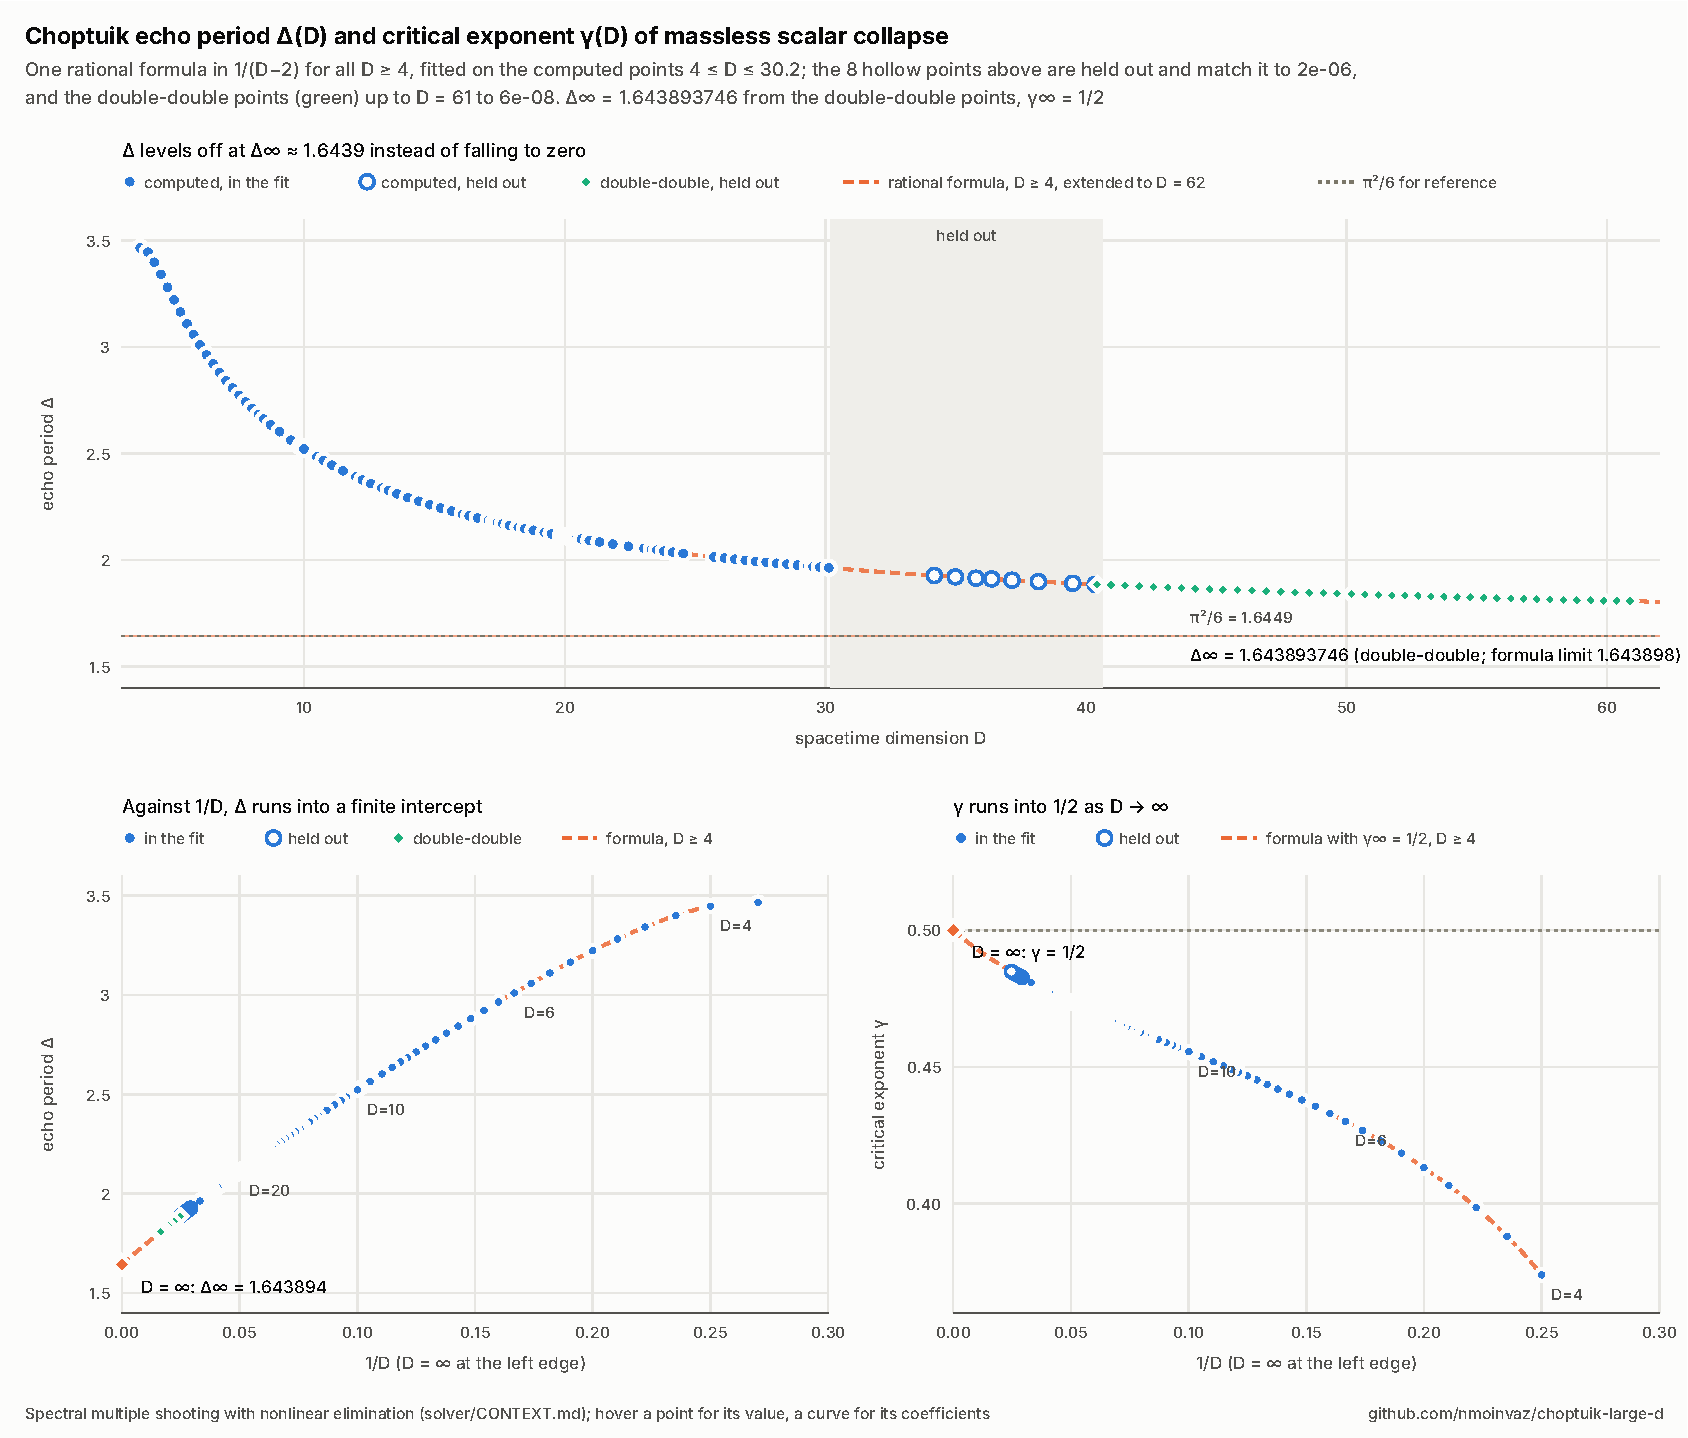
\includegraphics[width=\linewidth]{../figures/delta.pdf}
\caption{$\Delta(D)$ and $\gamma(D)$ with the rational formula~\eqref{eq:formula} (dashed), fitted on
$4 \le D \le 30.2$; hollow points are held out, and green diamonds are double-double points up to $D = 61$.}
\label{fig:delta}
\end{figure}

\subsection{Comparison with published values}
\label{sec:published}

At $D = 4$ the formula gives $\Delta = 3.4454524$ and $\gamma = 0.3739610$, in agreement with
$\Delta = 3.445452402(3)$~\cite{MartinGarciaGundlach2003} to about $10^{-8}$ and with
$\gamma = 0.373961 \pm 10^{-6}$~\cite{EckerEtAl2026} to about $10^{-7}$. Below $D = 4$ a cubic through the 47-mode
double-precision points at $D = 3.70$--$3.80$ puts the maximum of $\Delta$ at $D = 3.75570$, $\Delta = 3.466774$, in
agreement to $2\times10^{-6}$ with $D = 3.755726$, $\Delta = 3.466772$ of~\cite{EckerEtAl2026}.

At $D = 5$, Ref.~\cite{EckerEtAl2026} gives $\Delta = 3.22176$ and $\gamma = 0.41322$, which are $5.8\times10^{-5}$ and
$9.3\times10^{-5}$ above our values. Our $\Delta(5) = 3.2217019446$ comes from two independent codes: the
double-precision solver at 31, 39 and 47 Fourier modes ($3.221701945 \pm 7\times10^{-11}$ extrapolated) and the
double-double solver at $M = 48$ and $64$ collocation points ($3.22170194461806$, $3.22170194462672$), which agree to
$10^{-11}$. The published data of~\cite{EckerEtAl2026} (repository CriticalSpacetimeCrystal) show their $D = 5$ value
still moving by $-1.66\times10^{-4}$ between 256 and 512 modes, toward ours, in the range $D \gtrsim 4.8$ where they
note that their light-cone expansion order must be increased; their offset from our values grows smoothly from
$2.7\times10^{-7}$ at $D = 4$ (within their stated $\pm10^{-6}$) to $5\times10^{-4}$ at $D = 5.5$, and at $D = 3.7$ the two
agree to $8\times10^{-8}$, so there is no difference of convention. Their $\gamma$ list has no points for
$4.79 < D < 5.49$, where they report that their perturbation method fails, so their $\gamma(5)$ is not a direct
computation in the published data; ours, $0.41312694$ (stable to $10^{-7}$ across resolutions), agrees with Bland and
Kunstatter's $0.4131 \pm 0.0001$~\cite{BlandKunstatter2007}. Below $D = 4$, $\gamma$ extrapolated from our 47-mode points
suggests $\gamma(3.5) \lesssim 0.33$, against $0.349 \pm 0.003$ in~\cite{BlandEtAl2005}; our points there are
under-resolved, and this is an open check.

\subsection{Physical reading}

Each echo is a factor $e^{\Delta}$ smaller than the last: 31 at $D = 4$, 12 at $D = 10$, 5.2 at $D = \infty$. A
near-critical collapse makes about $\gamma\ln(1/|p-p^*|)/\Delta$ echoes before it forms a black hole or disperses, so
each further echo costs $\Delta/(\gamma\ln10)$ decimal digits of fine-tuning: 4.0 at $D = 4$, 2.4 at $D = 10$ and 1.43 at
$D = \infty$. In higher dimensions the echoes thus come closer together in scale and are cheaper to resolve. The shape
of the echo simplifies too (Fig.~\ref{fig:echo}): at $D = 4$ the centre slope is almost a square wave, with a third
harmonic 44\% of the first, while at $D = 60$ the third harmonic is 8\% of the first, and the $D = \infty$ theory of
Sec.~\ref{sec:selection} gives 5.5\%.

% =====================================================================================================
\section{The limit $D \to \infty$}
\label{sec:limit}

\subsection{Is the period analytic in $1/D$?}

Each model in Table~\ref{tab:analytic} is a polynomial in one variable, fitted at 60 digits on the cleaned
double-double points $10 \le D \le 45$ (or $\le 37.5$) and compared with every point above, up to $D = 60.1$, which it
never saw (the data snapshot when the table was made; Fig.~\ref{fig:heldout} uses all points to $D = 61.0$). Every
model fits its range to the level of the points, so the fit alone decides nothing; the unseen points do. Fitted on
$D \le 45$, the $1/D$ series predicts $\Delta$ fifteen units of $D$ ahead to $5\times10^{-13}$, while the series in
half-integer powers miss by 40 to 300 times more, and their limits jump with the degree. Adding one non-analytic term
($D^{-1/2}$, $D^{-3/2}$, $\ln D/D$, $\ln D/D^2$ or $e^{-D/4}$) to the degree-16 series changes neither the prediction nor
the limit, and the term's coefficient is not determined. The only structure the points show is a singularity on the
negative $D$ axis, near $D \approx -9$ to $-11$, which the rational formula represents by the zero of its denominator at
$D = -11.0$.

\begin{table}[t]
\caption{Held-out test of large-$D$ models (cleaned double-double points; snapshot $D \le 60.1$).}
\label{tab:analytic}
\footnotesize
\begin{ruledtabular}
\begin{tabular}{lllll}
Model & max residual, $10 \le D \le 45$ & worst error, $45 < D \le 60.1$ & fitted on $D \le 37.5$: worst error & limit \\ \hline
$1/D$, degree 16 & $4.1\times10^{-15}$ & $5.2\times10^{-13}$ & $4.2\times10^{-11}$ & 1.64389375 \\
$1/D$, degree 18 & $4.0\times10^{-15}$ & $1.8\times10^{-12}$ & $1.5\times10^{-10}$ & 1.64389377 \\
$1/(D-2)$, degree 18 & $4.0\times10^{-15}$ & $2.8\times10^{-12}$ & $7.9\times10^{-11}$ & 1.64389377 \\
$(D-2)^{-1/2}$, degree 20 & $3.9\times10^{-15}$ & $2.0\times10^{-11}$ & $3.9\times10^{-10}$ & 1.636 \\
$D^{-1/2}$, degree 20 & $3.8\times10^{-15}$ & $1.6\times10^{-10}$ & $6.2\times10^{-9}$ & 1.547 \\
\end{tabular}
\end{ruledtabular}
\end{table}

\begin{figure}[t]
\centering
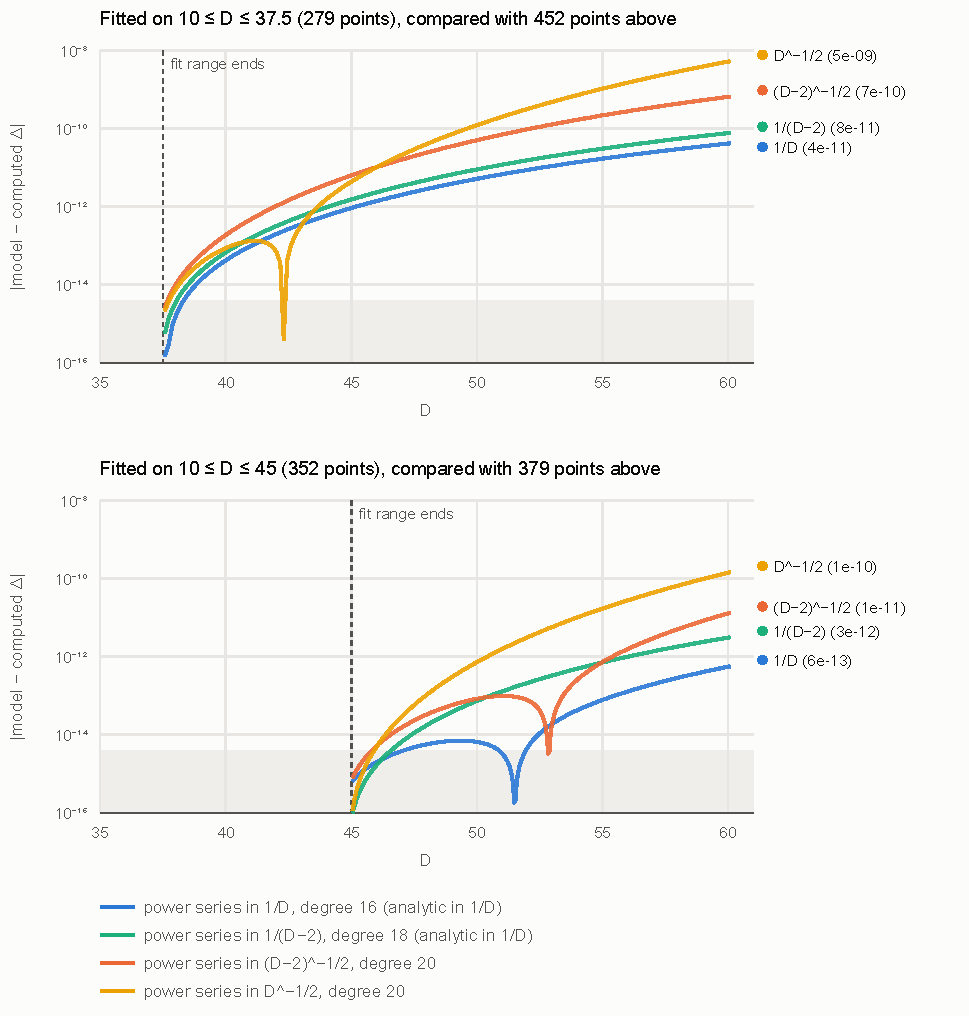
\includegraphics[width=0.8\linewidth]{../figures/heldout.pdf}
\caption{$|\text{model} - \text{computed}\ \Delta|$ on every double-double point above the fitted range, for fits on
$10 \le D \le 37.5$ (top) and $10 \le D \le 45$ (bottom); shaded: the level of the points.}
\label{fig:heldout}
\end{figure}

\subsection{The limit and its error bar}

Fitted on all cleaned points, power series in $1/D$ of degree 16--20 and in $1/(D-2)$ of degree 18--20 fit to the
noise and give limits from $1.643893744$ to $1.643893752$ (snapshot $D \le 60.1$) and from $1.643893745$ to
$1.643893752$ (all 823 cleaned points to $D = 61.03$). Over 48 choices of model ($1/D$, $1/(D-2)$), degree, fit range
and cleaning, the limit ranges over $1.643893744$--$1.643893763$; fitting on $D \le 45$ alone pins it only to
$2.5\times10^{-7}$. Hence, if $\Delta$ is analytic in $1/D$,
\begin{equation}
\Dinf = 1.64389375 \pm 1.5\times10^{-8}, \qquad \omega_\infty = 2\pi/\Dinf = 3.82213589 \pm 4\times10^{-8},
\label{eq:dinf}
\end{equation}
and $\Delta(D) \approx \Dinf + 10.37/n + \dots$. The $\pm1.5\times10^{-8}$ is a spread over fit choices, not an error
with a stated coverage, so we tested it on synthetic data with a known limit: the real $D$ grid, noise and junk points
like the real ones, and added structures ranging from a distant pole to a complex pole pair and a logarithmic branch
point near the data, plus one term outside the fitted model class. In all six cases the 48 fits put the known limit
inside their range, with the centre $0.8$--$0.9\times10^{-8}$ above it, so the bar holds and the quoted centre is
probably high by about $10^{-8}$. Analyticity is the natural default, since the large-$D$ expansion of the equations has
no other scale, but it is not proven: as Sec.~\ref{sec:picture} explains, the period is selected by an effect that the
$1/D$ expansion does not see.

\subsection{The conjecture $\Delta \to 0$}

The conjecture $\Delta \to 0$~\cite{EckerEckerGrumiller2026,EckerEtAl2026} comes with no rate. Fitted on
$10 \le D \le 45$ and compared with $45 < D \le 61$: a power-law approach to 0, $D^{-p}$ times a series in $1/D$ with
$p \ge 0.01$, misses the held-out points by $6\times10^{-8}$ or more, against $7\times10^{-13}$ for the analytic series;
a series in $1/\ln D$ with zero limit misses them by $1.3\times10^{-11}$ and still gives $\Delta \approx 0.88$ at
$D = 10^{30}$; adding a $c/\ln D$ term to the analytic series gives $c \approx 4\times10^{-7}$ and leaves the limit at
$1.6438937$. A power-law approach to 0 with $p \ge 0.01$ is excluded; a logarithmic one is disfavoured but cannot be
excluded from $D \le 61$ alone, and neither can a crossover far beyond the data. Bland's hypothesis
$\Dinf = 5/2$~\cite{Bland2007} is excluded by $\Delta(14) = 2.29$ and decreasing.

\subsection{Candidate closed forms}

Five constants that a product search placed inside the window of the earlier double-precision estimate (about nine
such coincidences are expected by chance in that search), and four classical constants, were tested. Each was forced as
the limit of a power series in $1/D$ fitted on $10 \le D \le 45$ (degree 14 to 26) and compared with the 351 cleaned
points from 45 to 59.8 (Table~\ref{tab:cand}). All nine are excluded, given analyticity in $1/D$: the closest sits
$1.3\times10^{-5}$ from the limit, about 840 times its uncertainty, and every forced fit predicts the unseen points at
least 100 times worse than the free fit. Nor is $\Dinf$ a product of two of the listed constants with rational prefactor
$i/j$ ($i, j \le 12$) and exponents $\pm\tfrac12, \pm1, \pm2$ (514\,332 expressions; about 0.02 chance hits would be
expected in the window, so this null has little power). At eight known digits no integer-relation search could support
a closed form, so whether $\Dinf$ has one is open.

\begin{table}[t]
\caption{Candidate closed forms for $\Dinf$, forced as the limit: best held-out error and its ratio to the free fit.
$G$ is Catalan's constant, $j_{\nu,k}$ the $k$-th zero of $J_\nu$.}
\label{tab:cand}
\small
\begin{ruledtabular}
\begin{tabular}{llll}
Candidate & value & minus $\Dinf$ & held-out error (ratio) \\ \hline
none (free fit) & $1.64389375 \pm 1.5\times10^{-8}$ & & $4.7\times10^{-13}$ \\
$\tfrac57\sqrt{G}\,j_{0,1}$ & 1.6439747 & $+8.1\times10^{-5}$ & $6.2\times10^{-11}$ (130) \\
$\tfrac75(\ln2)^{-2}\pi^{-1/2}$ & 1.6440014 & $+1.1\times10^{-4}$ & $1.1\times10^{-10}$ (220) \\
$\tfrac72\sqrt{\ln2/\pi}$ & 1.6440152 & $+1.2\times10^{-4}$ & $1.3\times10^{-10}$ (270) \\
$\tfrac98\sqrt{j_{2,1}/j_{0,1}}$ & 1.6440207 & $+1.3\times10^{-4}$ & $1.4\times10^{-10}$ (290) \\
$\tfrac{10}{9}\sqrt{j_{0,1}/\ln3}$ & 1.6439063 & $+1.3\times10^{-5}$ & $5.4\times10^{-11}$ (110) \\
$\pi^2/6$ & 1.6449341 & $+1.0\times10^{-3}$ & $1.7\times10^{-9}$ (3500) \\
$2\pi/j_{1,1}$ & 1.6397880 & $-4.1\times10^{-3}$ & $7.0\times10^{-9}$ (15000) \\
$\sqrt e$ & 1.6487213 & $+4.8\times10^{-3}$ & $8.1\times10^{-9}$ (17000) \\
$(1+\sqrt5)/2$ & 1.6180340 & $-2.6\times10^{-2}$ & $4.4\times10^{-8}$ (92000) \\
\end{tabular}
\end{ruledtabular}
\end{table}

\subsection{The critical exponent tends to $1/2$}
\label{sec:gammainf}

Unconstrained fits of the double-precision $\gamma$ on $D \ge 8$--$12$ give $\gamma_\infty = 0.4996$--$0.4998$. The
double-double $\gamma$ pins the limit much more tightly. In free fits of $\lambda = 1/\gamma$ in powers of $1/n$,
$\lambda_\infty - 2$ falls by a factor of about 3.5 with each added power: on $D \ge 30$, $2.4\times10^{-4}$,
$6.7\times10^{-5}$, $1.9\times10^{-5}$, $5.5\times10^{-6}$ and $(1.6 \pm 2.2)\times10^{-6}$ for four to eight powers, with no
sign of levelling off (Fig.~\ref{fig:gamma}), and at every order fixing $\lambda_\infty = 2$ fits better than leaving it
free with the same number of parameters. So $\lambda_\infty = 2$ to about $10^{-6}$ and $\gamma_\infty = 1/2$ to about
$5\times10^{-7}$, with
\begin{equation}
\lambda = 2 + \frac{3.0324}{n} - \frac{34.3}{n^2} + \dots, \qquad \gamma = \frac12 - \frac{0.7581}{n} + \dots
\label{eq:lambda}
\end{equation}
(the $1/n$ coefficient is stable to about $10^{-3}$ across fit choices: $3.0313$--$3.0324$). At $D = 61$, $\gamma = 0.48935$, and the points
keep rising, which excludes the limit $0.466$ of the fit of~\cite{BlandEtAl2005}. The value $1/2$ itself is not new: it
is Rozali and Way's estimate~\cite{RozaliWay2018}, reported in~\cite{EckerEckerGrumiller2026,EckerEtAl2026}. Like
$\Dinf$, it is not fixed at any finite order of the $1/n$ expansion (Sec.~\ref{sec:allorders}); its explanation is in
Sec.~\ref{sec:r2shift}.

\begin{figure}[t]
\centering
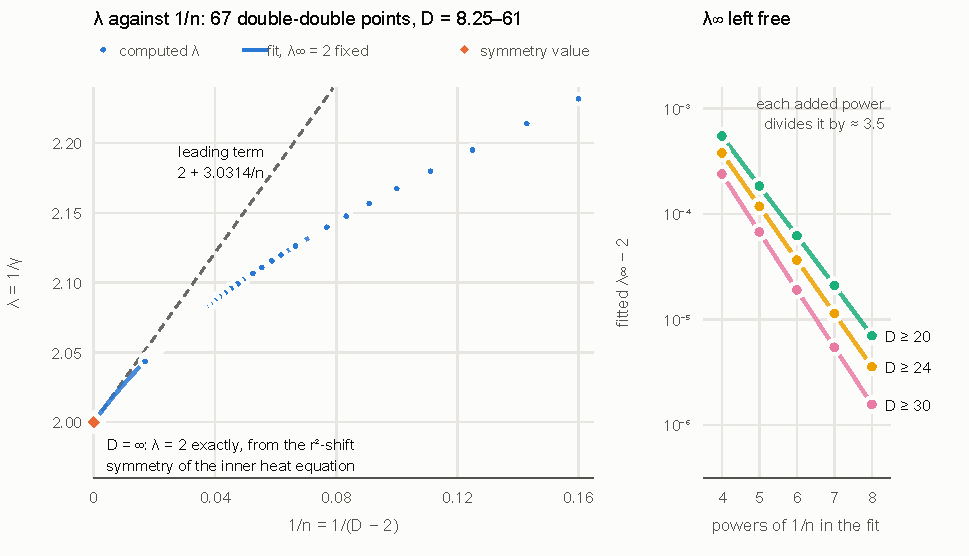
\includegraphics[width=\linewidth]{../figures/gamma.pdf}
\caption{Left: $\lambda = 1/\gamma$ against $1/(D-2)$ for 67 double-double points, with a fit fixing $\lambda_\infty = 2$ (solid,
over its range $D \ge 16$) and its leading term $2 + 3.03/n$ (dashed); at $D = \infty$, $\lambda = 2$ is exact, from the
$r^2$-shift symmetry of the inner heat equation (Sec.~\ref{sec:r2shift}). Right: with $\lambda_\infty$ left free, the
fitted $\lambda_\infty - 2$ falls about 3.5-fold per added power of $1/n$, for three fit ranges.}
\label{fig:gamma}
\end{figure}

\section{The large-$D$ picture}
\label{sec:picture}

The numerics fix $\Dinf$ and $\gamma_\infty$; this section asks where they come from in the equations. The theory is
developed, with proofs where they exist, in the companion paper~\cite{math}; here we state its results as physics and
give the numerical evidence for each.

\subsection{How the solution scales with $D$}
\label{sec:scaling}

On the double-double solutions at $D = 12$--$60$: $p \approx x F(\theta)/\sqrt n$ near the centre, and $p + m$ is
smaller by a further factor of order $1/n$; $c = 1 - O(1/n)$ and $b - 1 = (p^2+m^2)/(n-1)$ to about 3\%; near the light
cone $c$ stays within $10^{-3}$ of 1. The profile $F = \sqrt n\,\partial_x p(x = 0)$ converges as $D$ grows
(Table~\ref{tab:scaling}). So the field and its gravity weaken inside the light cone: the centre slope falls like
$2.72/\sqrt n$ and the departure of $c$ from 1 at the centre like $3.65/n$, and the last two columns of the table
approach the same limit, as the large-$D$ expansion requires ($c = 1 - \eps F^2(1-x^2) + \dots$). This scaling is forced
by one measured fact, $c - 1 = O(1/n)$: the $b$ equation then gives $b - 1 \approx (p^2+m^2)/(n-1)$, the $c$ equation
$c - 1 = O(p^2)$, so $p = O(n^{-1/2})$, and the $O(n)$ terms of the $p$, $m$ equations force $p + m = O(p/n)$. At
$D = \infty$ the echo inside the light cone is therefore a free scalar wave on flat space.

\begin{table}[t]
\caption{The echo profile $F = \sqrt n\,\partial_x p(0)$ and the strength of gravity at the centre on the double-double
solutions, and their $D = \infty$ extrapolations.}
\label{tab:scaling}
\small
\begin{ruledtabular}
\begin{tabular}{rlllll}
$D$ & first harmonic of $F$ & $|F_3/F_1|$ & $|F_5/F_1|$ & $n(1 - \langle c(0)\rangle)$ & $\langle F^2\rangle$ \\ \hline
20 & 3.480 & 0.130 & 0.024 & 3.021 & 6.162 \\
30 & 3.212 & 0.105 & 0.016 & 3.201 & 5.218 \\
40 & 3.086 & 0.093 & 0.012 & 3.304 & 4.804 \\
50 & 3.011 & 0.085 & 0.0097 & 3.372 & 4.568 \\
60 & 2.962 & 0.080 & 0.0085 & 3.421 & 4.416 \\
$\infty$ (extrapolated) & $\approx 2.72$ & 0.0549--0.0552 & 0.0032--0.0034 & $\approx 3.65$ & $\approx 3.7$ \\
\end{tabular}
\end{ruledtabular}
\end{table}

\subsection{A free wave cannot echo, and the period is selected beyond all orders}
\label{sec:allorders}

At leading order ($c = b = 1$) a single harmonic $e^{i\mu\theta}$ of the field, with $s = i\mu\omega$, solves
Gauss's hypergeometric equation: the solution regular at the centre is $p - m = x\,{}_2F_1\big(\tfrac{1+s}{2},
\tfrac{2+s}{2}; \tfrac{n+1}{2}; x^2\big)$, and by Gauss's connection formula~\cite{AbramowitzStegun} it contains, near the
light cone, the non-analytic branch $(1-x^2)^{n/2-1-s}$ with coefficient
\begin{equation}
C(n,s) = \frac{\Gamma\!\left(\frac{n+1}{2}\right)\Gamma\!\left(s+1-\frac n2\right)}{\Gamma\!\left(\frac{1+s}{2}\right)\Gamma\!\left(\frac{2+s}{2}\right)} ,
\label{eq:C}
\end{equation}
which is finite and non-zero for every real $\omega \ne 0$, odd $\mu$ and $n \ge 2$~\cite{math}. So a free wave that is
periodic in $\tau$ and regular at the centre is never analytic at the light cone: on its own it cannot echo, in any
$D \ge 4$. (The free wave equation in similarity coordinates was analysed in 3+1 dimensions by
Donninger~\cite{Donninger2008}, which contains the $D = 4$ case.) For the fundamental at $\omega_\infty$,
$|C| = 0.0121$, 0.0114, 0.0124, 0.0192, 0.0405 at $n = 18$, 38, 58, 200, 1000: small, through a factor of order
$e^{-\pi\omega/2}$, but never zero. Gravity has to cancel this coefficient harmonic by harmonic, and that cancellation
is what selects $\Delta$ and the profile $F$.

The $1/n$ expansion of the field equations never sees it. Within the scaling measured above (integer powers of $1/n$
after an overall $n^{-1/2}$ in the field), the expansion can be carried to all orders for \emph{any} periodic profile $F$
and \emph{any} period, regular at the centre and analytic at the light cone at every order~\cite{math}; the leading-order
part of this freedom, any periodic profile with any period, is in Ecker, Ecker and
Grumiller~\cite{EckerEckerGrumiller2026}. Numerically: substituting the expansion through third order into the exact
equations, with $F$ from the $D = 60$ solution, the relative residuals fall like $n^{-3}$ for $n = 50$--$800$, both for
$\omega_0 = 2\pi/1.64389$ and for a wrong $\omega_0 = 2\pi/1.4$. The same holds for growing perturbations
$e^{\lambda\tau}$ with any $\lambda$. So if $\Delta(D)$ and $\gamma(D)$ are analytic in $1/D$, their expansion coefficients
cannot be computed order by order from the field equations: they are selected by effects smaller than every power of
$1/n$. That is the exponential weakening of the selection seen in the solver (Sec.~\ref{sec:method}).
Non-perturbative, trans-series corrections in $1/D$ are familiar in large-$D$ gravity~\cite{EmparanHerzog2020}; here they
decide the period itself.

The non-analytic piece is a fast WKB mode, $e^{-n\Phi(x)}$ with $\Phi = \ln x - \tfrac12\ln(1-x^2)$, exponentially small
at fixed $x < 1$. Gravity acts on it at order one: along its characteristics it multiplies the mode by a factor that never
vanishes (about 40 over $0.72 \le x \le 0.9$ at the $D = \infty$ amplitude, checked by direct integration with errors
falling like $1/n$) and shifts its light-cone exponent by $\langle F^2\rangle \approx 3.7$, so an expansion in the wave
amplitude cannot capture the selection, and gravity cannot cancel the piece on its way to the light cone. Every
characteristic of the mode reaches the centre, where it is singular, so a solution regular at the centre carries none of
it inside the light cone, at any order of the WKB expansion. The late orders of the $1/n$ series locate its
origin~\cite{Dingle1973,math}: $C(n,s)$ is the Stokes multiplier of a mode born at infinite self-similar radius and switched
on across a Stokes line along $x > 1$ that ends at the light cone. The period is therefore decided outside the past
light cone, where the fast mode and the slow solution meet: at $x \sim \sqrt n$.

\subsection{The inner region: Rozali and Way's heat equation}
\label{sec:inner}

At $x \sim \sqrt n$ the expansion is not uniform: $\eps x^2F^2 = O(1)$, so gravity is of order one there, and fast and
slow modes are not separated. In physical variables this is the region $r = O(\sqrt n)$ at fixed $t$, which is Rozali
and Way's regime~\cite{RozaliWay2018} (they keep $r$ fixed and rescale time by $\sqrt D$). Put $\rho = r/\sqrt n$,
\begin{equation}
s = \frac{\rho^2}{2} = \frac{r^2}{2n}, \qquad p - m = \sqrt s\;Y, \qquad \sqrt n\,(p + m) = \sqrt2\,s\,S ,
\end{equation}
with $t$ the time and $c$ the lapse-type function as before. At leading order in $1/n$ the field equations
become~\cite{math}
\begin{equation}
Y_t = c\,S, \qquad S_t = c\,\Big(Y_s + \frac{Y^3}{4}\Big), \qquad c_s = \frac{c\,Y^2}{4},
\qquad\text{i.e.}\qquad Y_s = \frac1c\,\partial_t\Big(\frac1c\,\partial_t Y\Big) - \frac{Y^3}{4},
\label{eq:heat}
\end{equation}
with $b - 1 = (p - m)^2/(2n)$: a nonlinear heat equation in which $s = r^2/(2n)$ plays the role of time and $t$ that of
space, with no large parameter left. These are Rozali and Way's leading-order large-$D$ equations: with their $r$,
$\tau = \sqrt D\,t$ and lapse factor $1 - \delta_0$ identified with our $\rho$, $t$ and $c^2$, their equations read
$\phi_s = c^{-1}\partial_t(c^{-1}\phi_t)$ and $c_s = \phi_t^2/c$, and $Y = 2\phi_t/c$, $S = Y_t/c$ satisfy
Eqs.~\eqref{eq:heat} identically (checked symbolically). Rozali and Way noted this parabolic character, with space and
time swapped. A discretely self-similar solution of Eqs.~\eqref{eq:heat} depends on $\xi = \rho/(-t) = x/\sqrt n$ and
$\theta$; its formal series at $\xi = 0$ reproduces the top-degree terms of the outer $1/n$ expansion (to
$2\times10^{-13}$ at orders 1--10). Two familiar objects appear. The fast mode of the outer region,
$e^{-n/(2x^2)} = e^{-t^2/(4s)}$, is the heat kernel. And without gravity the inner problem is Weber's (Hermite's)
equation, whose classical Stokes constant~\cite{DLMF} reproduces $C(n,s)$ at large $n$ (the ratio to Eq.~\eqref{eq:C} is
$1.00014$ at $n = 10^5$), so the light-cone obstruction of Sec.~\ref{sec:allorders} is a property of this $n$-free
problem. What this work adds to Rozali and Way's equations is the discretely self-similar problem posed on them: the
selection rule (Sec.~\ref{sec:selection}) and the $r^2$-shift argument for $\gamma_\infty$, which we turn to now.

\subsection{The $r^2$-shift and $\gamma_\infty = 1/2$}
\label{sec:r2shift}

Equations~\eqref{eq:heat} contain no explicit $s$ or $t$. They are invariant under $t$-translation, $s$-translation, the
scaling $(t, s, Y, S) \to (at, a^2s, Y/a, S/a^2)$, and the time reparametrizations $t \to T(t)$, $c \to T'c$, which are
gauge. A self-similar solution is invariant under (a discrete subgroup of) the scaling, and a continuous symmetry of
scaling weight $k$ acting on it produces a linear perturbation $\propto e^{k\tau}$, because $\partial_t \propto e^{\tau}$
and $\partial_s \propto e^{2\tau}$ at fixed $\xi$, $\theta$. The $t$-translation ($k = 1$) is the familiar $\lambda = 1$
mode, a shift of the time of the singularity. The $s$-translation ($k = 2$) gives $\lambda = 2$. It moves the lapse at the
centre, which the normalization $c = 1$ there forbids, but composed with the time reparametrization
$t \to t - e^{\tau}P(\theta)$, where $P + \omega P' = -2F^2$, it leaves the centre lapse alone. The combination is an exact
perturbation of the $D = \infty$ inner solution with $\lambda = 2$, regular at the centre~\cite{math}. As a check, a
perturbation recursion with gravity that builds in nothing about symmetries, run at $\lambda = 2$, reproduces the mode to
$10^{-180}$ in every resolved harmonic, while $\lambda = 1.9$ or $2.1$ miss by 7.5\% at the third order. Because the mode
is the derivative of a family of exact solutions (shifted and reparametrized copies of the background), its fast-mode
Stokes multipliers vanish whenever the background's do~\cite{math}: if the selection rule of Sec.~\ref{sec:selection} picks
the background, $\lambda = 2$ is one of its growth rates, with no transcendental condition involved.

The mode is physical, not gauge: the reparametrization is pure gauge and $t$-translation only shifts the accumulation
time, but $s$-translation shifts $r^2$, with $r$ the areal radius. In the inner region critical collapse is diffusion in
$s = r^2/(2n)$, and the unstable mode moves the solution along $s$. A supercritical evolution therefore forms its horizon
at $r_{\rm BH}^2 \propto p - p^*$, so $r_{\rm BH} \propto (p - p^*)^{1/2}$ and $\gamma_\infty = 1/2$: the discretely
self-similar counterpart of Rozali and Way's estimate~\cite{RozaliWay2018}, which came from the divergence radius of their
oscillating solutions. This also explains why $\lambda_\infty$ is a simple number while $\omega_\infty$ is not: $\omega$ is
fixed by the vanishing of a Stokes multiplier, $\lambda$ by a symmetry. The statement is conditional: \emph{if the
$D = \infty$ critical solution is selected by the rule of Sec.~\ref{sec:selection}, has no unstable mode other than
$\lambda = 2$ and the gauge mode $\lambda = 1$, and $\lambda(D)$ is continuous at $1/n = 0$, then $\gamma_\infty = 1/2$.}
The uniqueness of the unstable mode at $D = \infty$ is not shown. At finite $D$ the outer region and the $1/n$
corrections to Eqs.~\eqref{eq:heat} depend on $r$ explicitly, so the symmetry is broken and the mode survives as an
ordinary unstable mode with $\lambda = 2 + O(1/n)$; the data give $2 + 3.0324/n$ [Eq.~\eqref{eq:lambda}], a coefficient
that would need the $O(1/n)$ inner equations.

\subsection{The selection rule at $D = \infty$}
\label{sec:selection}

The $D = \infty$ form of the condition that the solution be analytic at the light cone is conjectured to
be~\cite{math}: \emph{the $D = \infty$ critical solution is the discretely self-similar solution of the inner
problem~\eqref{eq:heat}, regular at the centre, whose fast-mode Stokes multipliers vanish.} That is one complex condition
per odd harmonic, for unknowns that are the harmonics of the profile $F$ (less one phase) and $\omega$, so the count
balances; it uses no input from finite $D$. Without gravity it reduces to $C = 0$, which has no solution, so the
selection is gravity's doing even at $D = \infty$. The companion paper states the hypotheses under which the rule should
follow from analyticity at the light cone, and the points where a proof is still missing~\cite{math}. Here we list what
the rule, evaluated numerically on the $D = \infty$ equations alone, reproduces (Figs.~\ref{fig:selection}
and~\ref{fig:spectrum}).

\emph{The shape of the echo.} With the higher-harmonic multipliers tuned to zero at the amplitude $A = 2.72$ and
$\omega = \omega_\infty$, the profile has $|F_3/F_1| = 0.0551$ and $|F_5/F_1| = 0.00314$; the double-double solutions at
$D = 20$--$60$, extrapolated in $1/n$, give $0.0549$--$0.0552$ and $0.0032$--$0.0034$ (Table~\ref{tab:scaling}). The tuned
ratios of successive harmonics are nearly the same for every harmonic, $|F_{\nu+2}/F_\nu| \approx 0.063$, so the decay
rate per harmonic of the profile should level off near 1.4 as $D \to \infty$ rather than keep growing; the measured
ratios ($\nu = 1, \dots, 9$) extrapolate to a rate of 1.3--1.45 (not fully converged). The $D = \infty$ echo profile is
then not an entire function of $\theta$: it has singularities at a finite distance, $|\mathrm{Im}\,\theta| \approx 1.4$,
from the real axis. The same relation evaluated at each $D$'s own amplitude and $\omega$ (a heuristic) tracks the measured
$|F_3/F_1|$ at $D = 20$--$60$ to within $0.004$--$0.006$.

\emph{The period, without truncation.} Expanding the harmonic-1 multiplier in powers of $A^2$, with every harmonic kept
exactly at each order, to twelve orders, its zero becomes real at $\omega/\omega_\infty = 0.9999$--$1.0001$ (best
estimates; two families of estimators approach from opposite sides and bracket it in $0.99915$--$1.00011$), at amplitude
$A_0 = 2.720$, where the solutions extrapolate to 2.70--2.72. So the rule gives
\begin{equation}
\Dinf = 1.6439 \pm 0.0002
\end{equation}
from the $D = \infty$ inner equations alone, against $1.64389375$ from the finite-$D$ solutions. The $\pm0.0002$ is the
range of the estimators, not an error bound; whether the remaining $10^{-4}$ closes needs more orders.

\emph{The truncation sequence.} Keeping only $M$ harmonics in the profile, the full set of conditions selects
$\omega/\omega_\infty - 1 = -22\%$, $+1.56\%$ and $-0.077\%$ for $M = 1$, 3 and 5 ($\Delta$ 29\% above, 1.5\% below and
$0.077\%$ above $\Dinf$), alternating in sign and shrinking fifteen- to twentyfold per added pair of harmonics. Harmonic
truncation is not a controlled approximation here (the linear multipliers grow like $e^{\pi|\nu|\omega/2}$ with the
harmonic $\nu$), which is why the untruncated expansion above is the primary estimate. The multipliers were computed by
two implementations that share no code (lateral solutions on either side of the Stokes line, and Borel--Darboux fits in
ball arithmetic); at $M = 5$ and $(A, \omega) = (2.72, \omega_\infty)$ the first gives $F_3/F_1 = 0.05486 + 0.00541i$ and
$F_5/F_1 = 0.00309 + 0.00054i$, against the amplitude expansion's $0.05482 + 0.00543i$ and $0.00310 + 0.00056i$. For the
one-harmonic truncation, whose zero is not the physical one, the companion paper gives a computer-assisted proof,
assuming Braaksma's summability theorem and following the template of Baldom\'a et al.~\cite{BaldomaEtAl2023}, that the
selection condition has exactly one zero in a small box around it, and that it is simple~\cite{math} (Reiterer and
Trubowitz gave a computer-assisted existence proof of the $D = 4$ critical solution
itself~\cite{ReitererTrubowitz2019}).

The matter models of Sec.~\ref{sec:matter} give two further, truncation-free tests of the rule.

\begin{figure}[t]
\centering
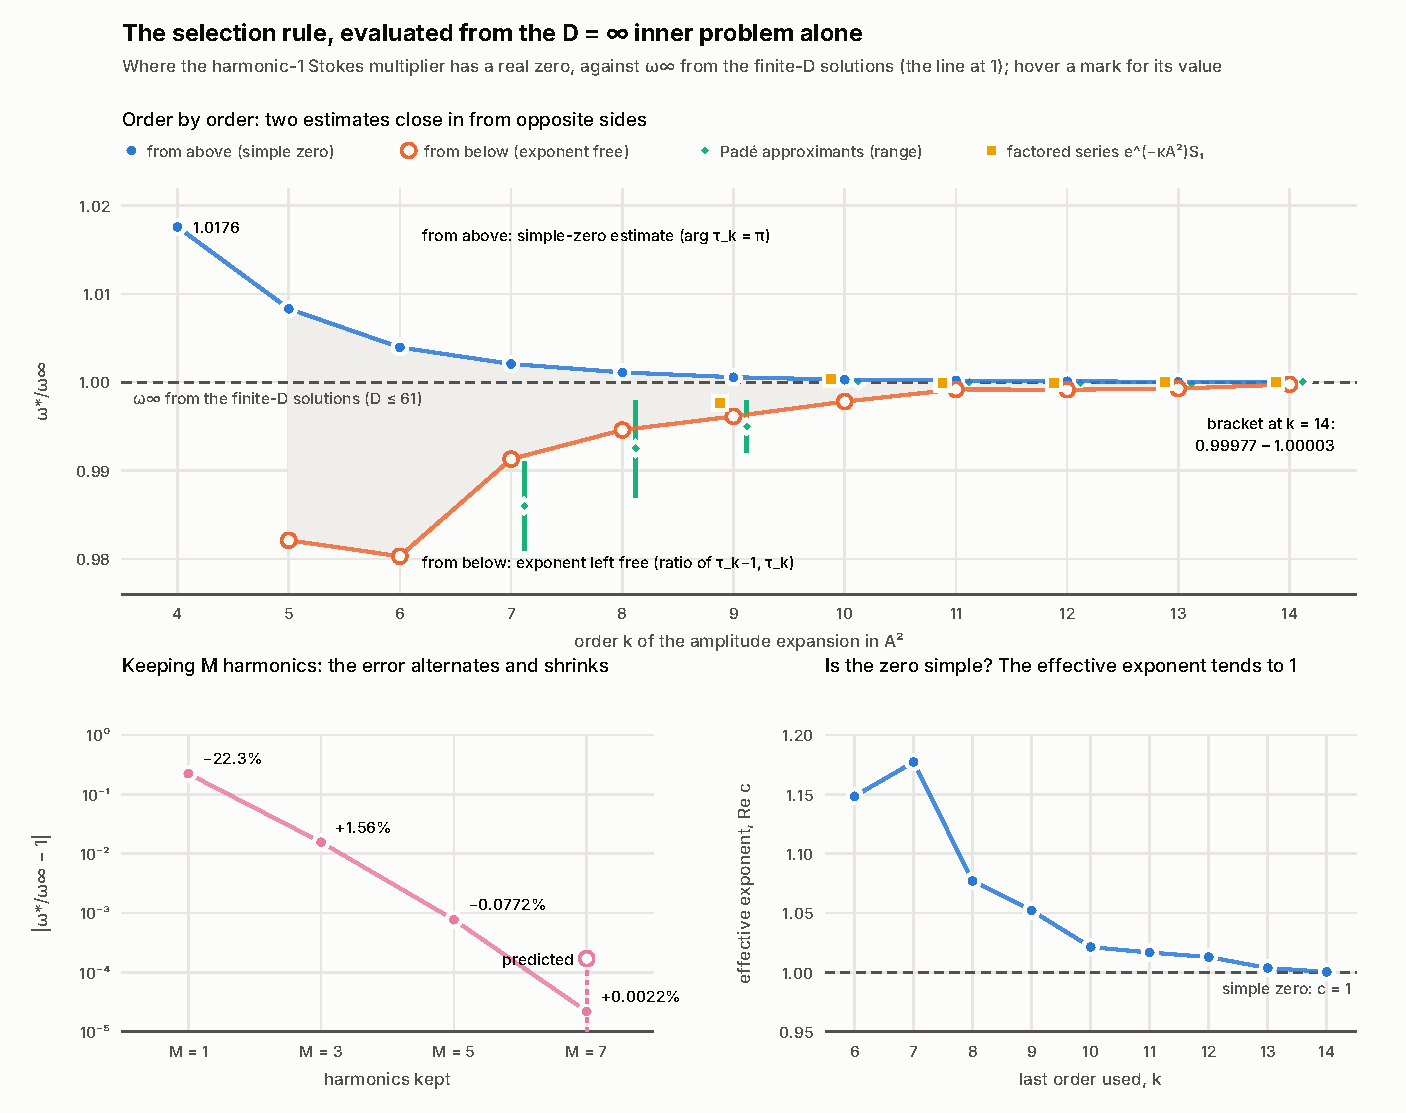
\includegraphics[width=\linewidth]{../figures/selection.pdf}
\caption{The selection rule evaluated from the $D = \infty$ inner problem alone. Top: where the harmonic-1 multiplier has
a real zero, order by order in the amplitude expansion; simple-zero estimates from above, floating-exponent estimates from
below, Pad\'e ranges and a factored series inside the shaded bracket, which narrows onto $\omega_\infty$ from the
finite-$D$ solutions (dashed). Bottom left: the truncated route, $|\omega^*/\omega_\infty - 1|$ for $M = 1$, 3, 5
harmonics (alternating in sign) and a prediction for $M = 7$. Bottom right: the effective exponent of the zero tends to 1,
a simple zero.}
\label{fig:selection}
\end{figure}

\begin{figure}[t]
\centering
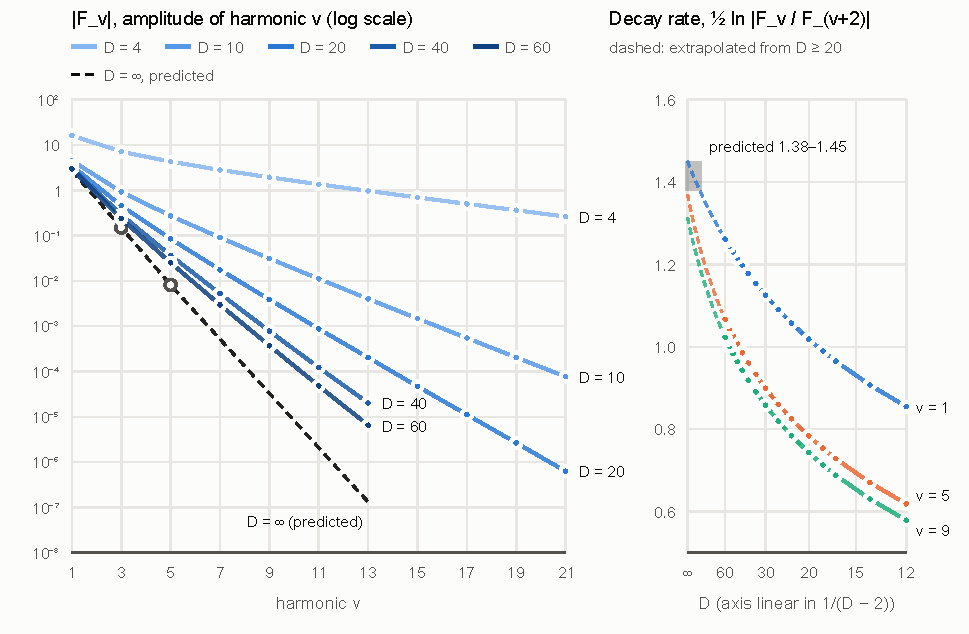
\includegraphics[width=\linewidth]{../figures/spectrum.pdf}
\caption{Left: amplitude $|F_\nu|$ of each odd harmonic of the echo profile for $D = 4$--$60$ and the $D = \infty$
prediction of the inner problem (dashed; beyond $\nu = 5$ the leading-order ratio, conjectured). Right: the decay rate
per harmonic, $\frac12\ln|F_\nu/F_{\nu+2}|$, against $1/(D-2)$, with extrapolations from $D \ge 20$ and the predicted
$D = \infty$ band.}
\label{fig:spectrum}
\end{figure}

\subsection{The next-to-leading-order condition of Ref.~\cite{EckerEckerGrumiller2026}}
\label{sec:eeg}

Ecker, Ecker and Grumiller use the same gauge: their $f = \alpha/a$ is our $c$, with $f = 1$ at the self-similarity horizon
$x = 1$, and their profile is $\beta(\tau) \approx \sqrt{2/n}\,F(\omega\tau)$. At next-to-leading order they require
$f \le 1$ near the horizon at the zeros of $\beta$, which leads to their Eq.~(20); in our variables the condition is
$\omega^2F'' + 3\omega F' = 0$ at the zeros of $F$. This condition does not select $\Delta$. The inequality $f \le 1$
holds for every regular solution, whatever the period: from $xb_x = b(p^2+m^2) - (n-1)b(b-1)$ with $b(0) = 1$, $b$ can
never drop below 1, so $xc_x = (n-1)c(b-1) \ge 0$ and $c \le c(1) = 1$. In the large-$D$ expansion, near a zero of $F$,
\begin{equation}
b - 1 = 2\eps^2x^2F(\theta - \delta\theta)^2 + 2\eps^4\omega^2x^4F'^2 + \dots, \qquad
\delta\theta(x) = -\eps\omega x^2\,\frac{3F' + \omega F''}{2F'},
\end{equation}
so the next-to-leading-order term is the cross term of a square whose square term arrives one order later. The
double-double solutions bear this out: they violate the condition [$(\omega^2F''+3\omega F')/(3\omega F') = 0.98$--$1.06$
at $D = 12$--$60$, since $F$ is nearly antisymmetric about its zeros], the zero line of $p - m$ tilts as $\delta\theta(x)$
predicts (measured over predicted at $x = 1$: 0.69 to 0.88 for $D = 20$--$60$), and the maximum of $c$ at the centre
approaches $1 - (\eps^3/2)\omega^2F'^2$, their Eq.~(22) in this scaling (ratio 0.36 to 0.86). The same condition is used
by Lai and Wen~\cite{LaiWen2026}, who take it to select the period; the argument applies to that use as well.

\section{Other matter at large $D$}
\label{sec:matter}

\section{Discussion}
\label{sec:discussion}

\section{How this work was done}
\label{sec:how}

\begin{thebibliography}{99}
\bibitem{math} N. Moinvaziri, The echo period of Choptuik's critical solution at large dimension: a selection rule and
a computer-assisted proof (in preparation).
\end{thebibliography}

\end{document}
